\section{Introduction}

\begin{figure}[t]
    \centering
    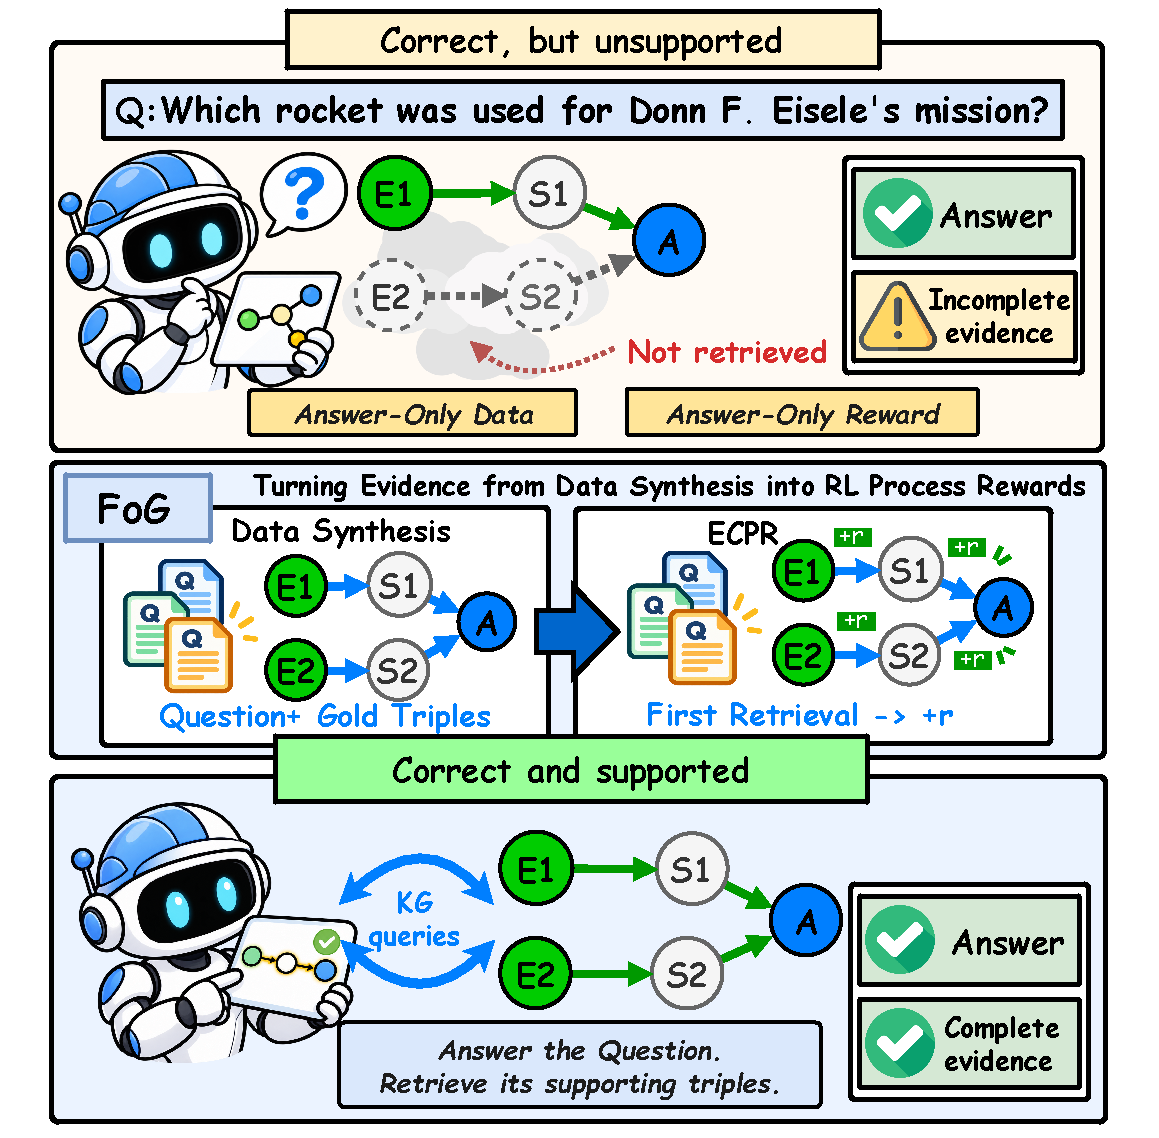
\includegraphics[width=1\linewidth]{figures/overview.pdf}
    \caption{\textbf{Motivation of FoG.}
    Answer-only training yields correct but unsupported answers, whereas FoG embeds supporting triples at synthesis and rewards their retrieval during RL training.}
    \label{fig:intro}
    \vspace{-5mm}
\end{figure}

Large language models (LLMs)~\citep{kimi,GLM,qwen,llama,gpt-4} increasingly answer factual questions from parametric knowledge, but remain difficult to trust on questions that require \emph{complex factual reasoning}~\cite{mirzadeh2025gsm,hu2024large,jullien2025knowledge,petroni2021kilt}. A correct answer is not necessarily a supported one: the model may answer from memory or surface cues while exposing little about \emph{why} the answer holds~\citep{hallucination_1,hallucination_2,nguyen2024direct}, which is problematic in high-stakes settings such as healthcare and law~\cite{cabello2024meg}, where users need evidence that they can check~\cite{sui2025fidelis,agrawal2024mindful}. Current LLM answers thus lie in a \emph{fog}: the answer is visible, yet the evidence behind it remains hidden.

Knowledge graphs (KGs)~\cite{roadmap} offer a natural way to clear this fog, since they store facts as verifiable triples. Existing KG-augmented methods follow two paradigms (Figure~\ref{fig:related_work}). \emph{Retrieval-based} methods~\citep{RoG,SubGraphRAG,GCR} retrieve triples, paths, or subgraphs and answer from them. \emph{Agent-based} methods~\citep{ToG,PoG,KG-R1,kg-agent} interact with the KG through a multi-turn ``think--act--observe'' process, and recent work trains them with reinforcement learning (RL)~\citep{KG-R1,KnowCoder-A1,KBQA-R1,SoG-R1}.

\begin{figure*}[t]
    \centering
    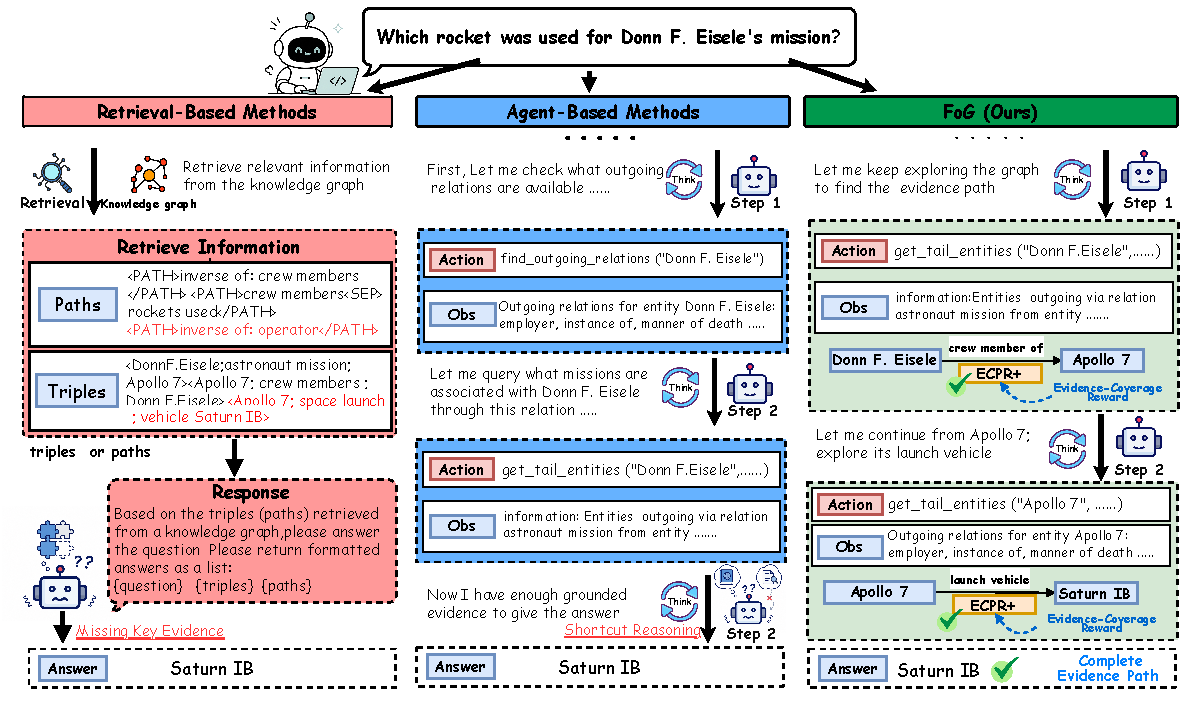
\includegraphics[width=1\textwidth]{figures/related_work.pdf}
    \caption{\textbf{Comparison of KG-augmented reasoning paradigms.}
    All three methods return the correct answer, but retrieval-based methods miss key evidence and agent-based methods answer after the first hop, whereas FoG retrieves every supporting triple of the answer.}
    \label{fig:related_work}
    \vspace{-3mm}
\end{figure*}

However, existing KG agents treat the KG only as a \textbf{source of answers} and overlook its role as a \textbf{source of evidence}. An LLM with no KG access can already answer many benchmark questions correctly, and even an RL-trained agent can answer correctly while retrieving only part of the supporting triples. We identify two causes. First, \emph{training data carries answers but not evidence}: most KGQA datasets annotate answers and at most logical forms~\cite{cwq,webqsp,grailqa}, and recovering the supporting triples afterwards requires enumerating and verifying paths for every question. Second, \emph{training rewards check the answer but not the evidence}: most rewards score only the final answer or whether the KG returns it~\cite{KG-R1,Plan-Then-retrieve,GraphWalker,KnowCoder-A1,KBQA-R1}, so a trajectory that reaches the answer through part of the evidence earns as much as one that retrieves all of it. The process rewards that go further depend on an LLM judge or on gold paths recovered for every question~\cite{KG-Hopper,EoG}, both of which are costly. Both causes trace back to one bottleneck: \emph{evidence is expensive to recover once a question has been written}.

To remove this bottleneck, we propose \textbf{FoG} (Figure~\ref{fig:intro}), a framework that trains KG agents to retrieve the evidence behind their answers. Our key observation is that evidence is hard to recover after a question is written but can be embedded when the question is constructed and then rewarded during training. First, \textbf{evidence-grounded synthesis} recursively hides the explicit entities of a seed question behind verifiable sub-questions, so every question carries its supporting triples. Second, a \textbf{KG interaction agent} answers through multi-turn KG queries and records every triple that the KG returns. Lastly, during RL training, an \textbf{evidence-coverage process reward} (ECPR) gives a dense reward to each turn that first retrieves one of these supporting triples. Our contributions are as follows:
\begin{itemize}[leftmargin=*,itemsep=0pt,topsep=2pt]
    \item We distinguish two roles of the KG and show that existing training data and rewards serve it only as a source of answers, not of evidence.
    \item We propose FoG, which embeds supporting triples into synthetic questions and rewards their retrieval through ECPR, so the dense reward comes from data synthesis with no LLM judge or extra annotation.
    \item On three benchmarks, 3B--4B FoG agents outperform larger baselines in accuracy and evidence coverage, and transfer zero-shot across KGs.
\end{itemize}
